\documentclass[twoside, 12pt, letterpaper]{article}

\ifx\pdfoutput\undefined
  \usepackage[dvips]{graphicx} % LaTeX
%  \DeclareGraphicsExtensions{.eps}
\else
  \usepackage[pdftex]{graphicx} % pdfLaTeX
  \DeclareGraphicsExtensions{.pdf}
  \usepackage{hyperref}
  \hypersetup{
       pdfauthor = {Marc Salzmann},
       pdftitle = {WRF-Chem/KPP},
       pdfsubject = {},
       pdfkeywords = {},
}
\fi



\usepackage{html}
\usepackage{natbib}
\usepackage[nottoc]{tocbibind}




%\newcommand{\clearemptydoublepage}{\newpage{\pagestyle{empty}\cleardoublepage}}
\oddsidemargin=-0cm
\evensidemargin=-0.5cm
\textwidth=16.5cm

%p. 148 of big meat dog latex companion
\usepackage{float}
%%\floatstyle{boxed}
\newfloat{File}{thp}{loa}
\floatname{File}{\small \sf Example File}


\newsavebox{\fminibox}
\newlength{\fminilength}
\newenvironment{fminipage}[1][\linewidth]
 {\setlength{\fminilength}{#1}%
   \begin{lrbox}{\fminibox}\begin{minipage}{\fminilength}}
{\end{minipage}\end{lrbox}\noindent\fbox{\usebox{\fminibox}}}





\newenvironment{V0}%
  {\begin{list}{}{\renewcommand{\makelabel}[1]{\hfil $\bullet$}%
   %\vspace{-2mm}%
  %\setlength{\itemsep}{-\parsep+3pt}
  \setlength{\leftmargin}{6mm}}}%
 {\end{list}}

\newenvironment{V1}%
  {\begin{list}{}{\renewcommand{\makelabel}[1]{\hfil \tiny $\bullet$}%
   \vspace{-2mm}%
  \setlength{\itemsep}{-\parsep}
  \setlength{\leftmargin}{3mm}}
 % \vspace{-2mm}%
}%
 {\end{list}}






\begin{document}
\title{\Large \bf WRF-Chem/KPP Coupler (WKC)\\ \vspace*{4mm} Version 1.0.0 User's and Developer's Guide\vspace*{-4mm}}
\author{Marc Salzmann\\ salzmann@mpch-mainz.mpg.de}
%\author{{Marc~Salzmann} \\ \\ Max-Planck-Institute for Chemistry \\ Department of Atmospheric Chemistry \\ Mainz, Germany \\ salzmann@mpch-mainz.mpg.de.}
\maketitle
\tableofcontents
\vfill
\pagebreak
%\clearemptydoublepage
\section{Preface}
{\bf WKC} is an acronym for the {\bf W}RF-Chem/{\bf K}PP {\bf C}oupler. For an introduction to WKC see the extended abstract to Presentation (6.4) by Salzmann and Lawrence, 2006 WRF-User Workshop \htmladdnormallink{\tt (chem/KPP/documentation/abstr\_wkc.pdf)}{ext_abstr_wkc.pdf}. Documentation for {\bf KPP} ({\bf K}inetic {\bf P}re{\bf P}rocessor) is e.g. provided at Adrian Sandu's homepage:
\begin{center}
\htmladdnormallink{http://people.cs.vt.edu/~asandu/Software/Kpp/}{http://people.cs.vt.edu/~asandu/Software/Kpp/}.
\end{center}
References for KPP are among others \cite{dam02, sandu03,s+s06} (please give credit when using KPP generated code). KPP and WKC are distributed under the \htmladdnormallink{GNU General Public License (GPL)}{http://www.gnu.org/copyleft/gpl.html}. {\bf At this stage, Version 1.0.0 of WKC and its documentation are still a $\beta$ releases and are recommended for friendly users/developers only.} Constructive comments and suggestions regarding the coupler and/or this documentation are welcome. Only a limited number of all KPP features are available for use with WKC, but more features may be added in the future. 



\section{Requirements for running KPP}
 KPP requires {\tt flex}, {\tt yacc}, and {\tt sed} to be installed. The 
 path to the {\tt flex} library (either {\tt libfl.a} or {\tt libfl.sh}) is specified by the environment variable {\tt FLEX\_LIB\_DIR}. The default path is {\tt /usr/lib}. If {\tt libfl.a} (or {\tt libfl.sh}) is not located in {\tt /usr/lib} on your system {\tt FLEX\_LIB\_DIR} should be set prior to compiling WRF-Chem. The C compiler is set by {\tt configure\_kpp} based on the settings in {\tt configure.wrf}. 
%For details regarding the installation of KPP consult \htmladdnormallink{Section 1 of the KPP User's manual}{kpp_UserManual.pdf}.

\section{Compiling and Running KPP together with WKC}
WKC and KPP are compiled and executed automatically when WRF-Chem is compiled. WKC copies the KPP generated code to the {\tt chem} directory and automatically  modifies the {\tt Makefile} in the {\tt chem} directory, so that the KPP generated code is compiled into WRF-Chem. The KPP and WKC generated modules in the {\tt chem} directory contain the string {\tt \_kpp\_} in their file names. Running the {\tt clean} script removes these modules.   

\section{Using mechanisms already implemented with WKC}
KPP files for mechanisms which have already been implemented with WKC are located in subdirectories of {\tt chem/KPP/mechanisms}. The corresponding packages  are declared in the file {\tt Registry/Registry.EM\_CHEM} and contain the suffix ``{\tt \_kpp}'' in their name. In order to use one of these mechanisms inside WRF-Chem, set the {\tt chem\_opt} in the {\tt namelist.input} to the corresponding value (find out the number by browsing the {\tt Registry.EM\_CHEM}). 

\noindent The following mechanisms are currently available (thanks to Rainer Schmitz, University of Chile, who made the  KPP input files for these mechanisms available):
\begin{itemize}
\item RACM, \cite{sto97}.
\item RACM-MIM, \cite{gei03}.
\end{itemize} 

\noindent These WKC implemented mechanisms have {\tt chem\_opt $>$ 100}.
 See Section~\ref{sec:add_mech} on how to add additional mechanisms.


\section{Layout of WKC}
\begin{figure}[h]
  % don't type the extension (eps or pdf) of the graphics file here
  \begin{center}
  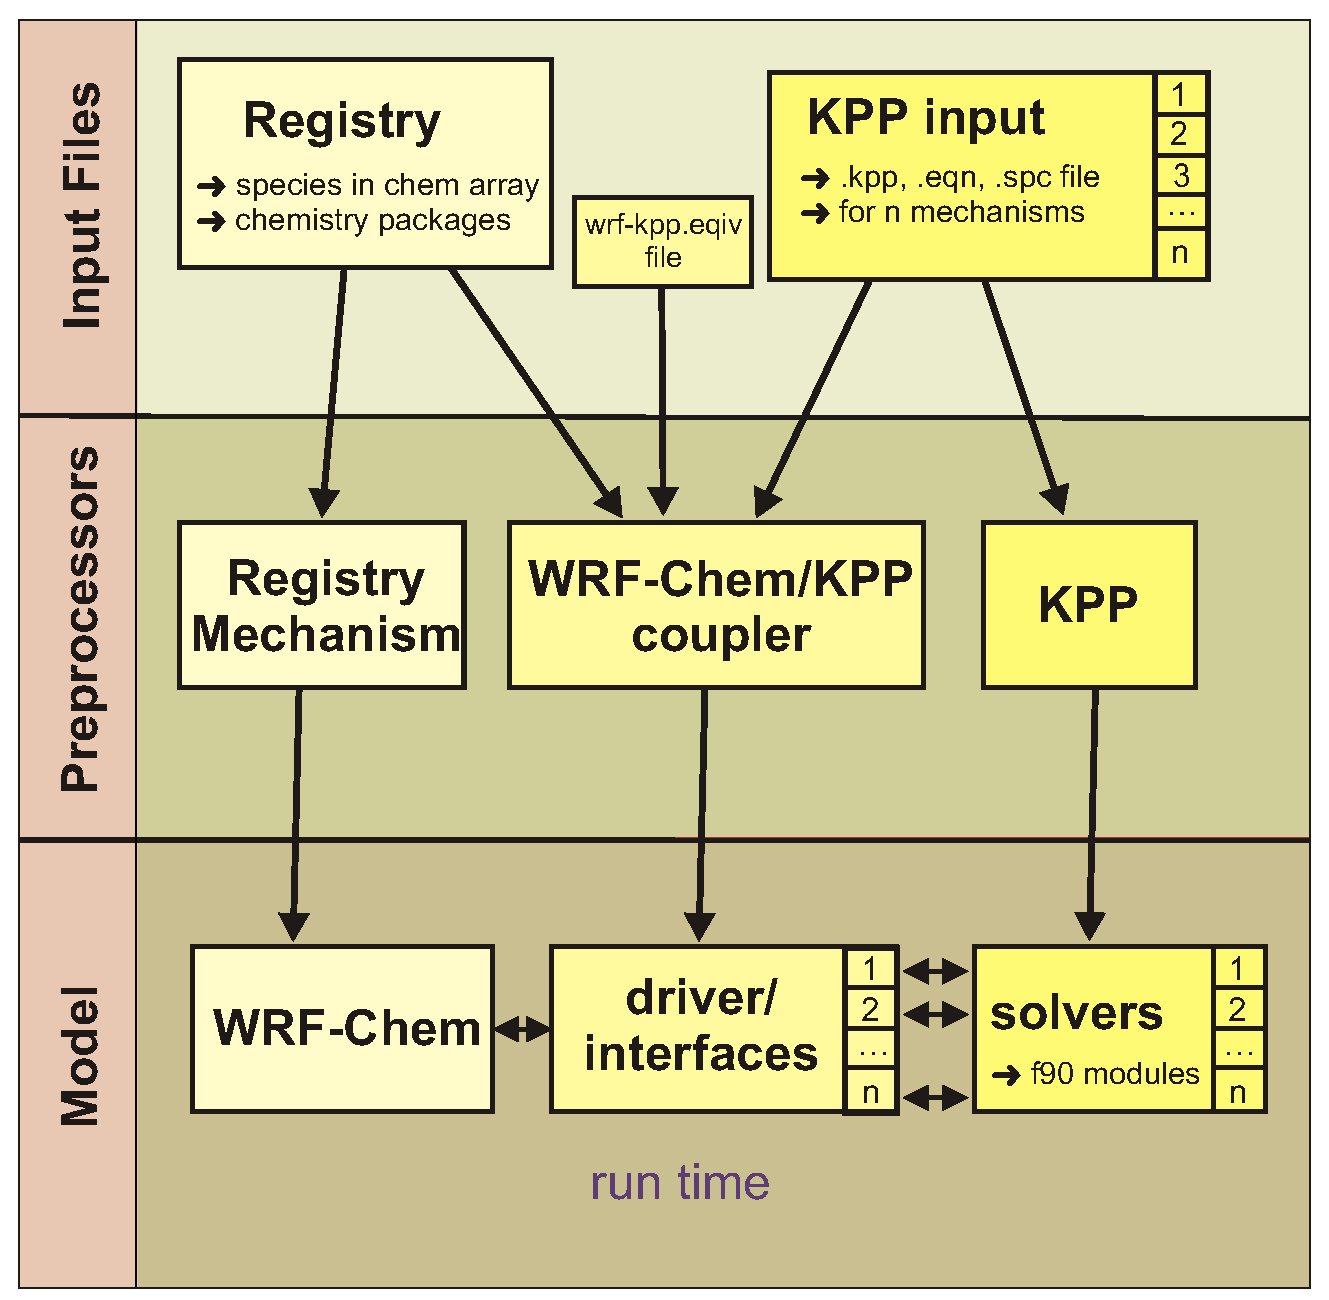
\includegraphics[width=11cm]{figs/wkc_schematic_2}  
  \end{center}
  \caption{\label{fig:schem} Schematic: Input files (ASCII), ``Preprocessors'' run during build time (written in C), and  WRF-Chem with coupled KPP solvers (written in Fortran 90.)}
\end{figure}

 WKC reads KPP species input files with suffix {\tt .spc} and the file {\tt Registry/Registry.EM\_CHEM} and automatically generates the Fortran 90 interface routines between WRF-Chem and the KPP generated code (see  Fig.~\ref{fig:schem}). It is in parts based on the WRF registry mechanism. The WKC related files are located in the {\tt chem/KPP} directory. This directory contains: 
\begin{itemize}
\item a subdirectory {\tt mechanisms} which holds directories with KPP input files for different mechanisms. 
\item a compile and a clean script for WKC (which are executed from the WRF-Chem compile script).
\item a version of KPP v2.1  in the {\tt kpp} subdirectory. This version of KPP was adapted to produce code which can directly be used with WRF-Chem  (using the {\tt \#WRF\_Conform} option in the .kpp file).
\item the source code of WKC in the {\tt util/wkc} subdirectory.
\item {\tt module\_wkpp\_constants.F} which allows to specify input to kpp such as RTOL and ATOL (likely to be extended in the future). 
\item a subdirectory {\tt inc} containing files which are included during compile time  (using  ``{\tt \#include}'' statements). The files in {\tt chem/KPP/inc}are not removed by the WKC clean script. Their purpose is to allow user modifications to WKC generated code. 
 \end{itemize} 
 
At the heart of WKC is the routine {\tt gen\_kpp.c}, which is located in the {\tt util/wkc} directory.




\section{Code produced by WKC, User Modifications}
The code produced by WKC is called from the chem\_driver (see schematic call tree in Fig.~\ref{fig:call}). Since parts of the code are generated automatically, manual changes will be lost when re-compiling WRF-Chem (as indicated by a warning in the header of the corresponding files). There are, however, a number of ``{\tt \#INCLUDE}'' preprocessor statements in the WKC generated code. The files included (in the {\tt .f} files) are located in the chem/KPP/inc directory. These files are not removed by the clean script and can be used to inline user supplied code. In case this should not be enough, there are two ways to edit automatically generated files permanently: The files can either be renamed in such a way that they won't be removed by the {\tt clean\_kpp} script, or the C code which generated the files (either KPP or WKC) can be edited. The latter is generally the better solution. However, the method of using include files in the {\tt chem/KPP/inc} directory is strongly recommended.     
  

\begin{figure}[h]
  % don't type the extension (eps or pdf) of the graphics file here
  \begin{center}
  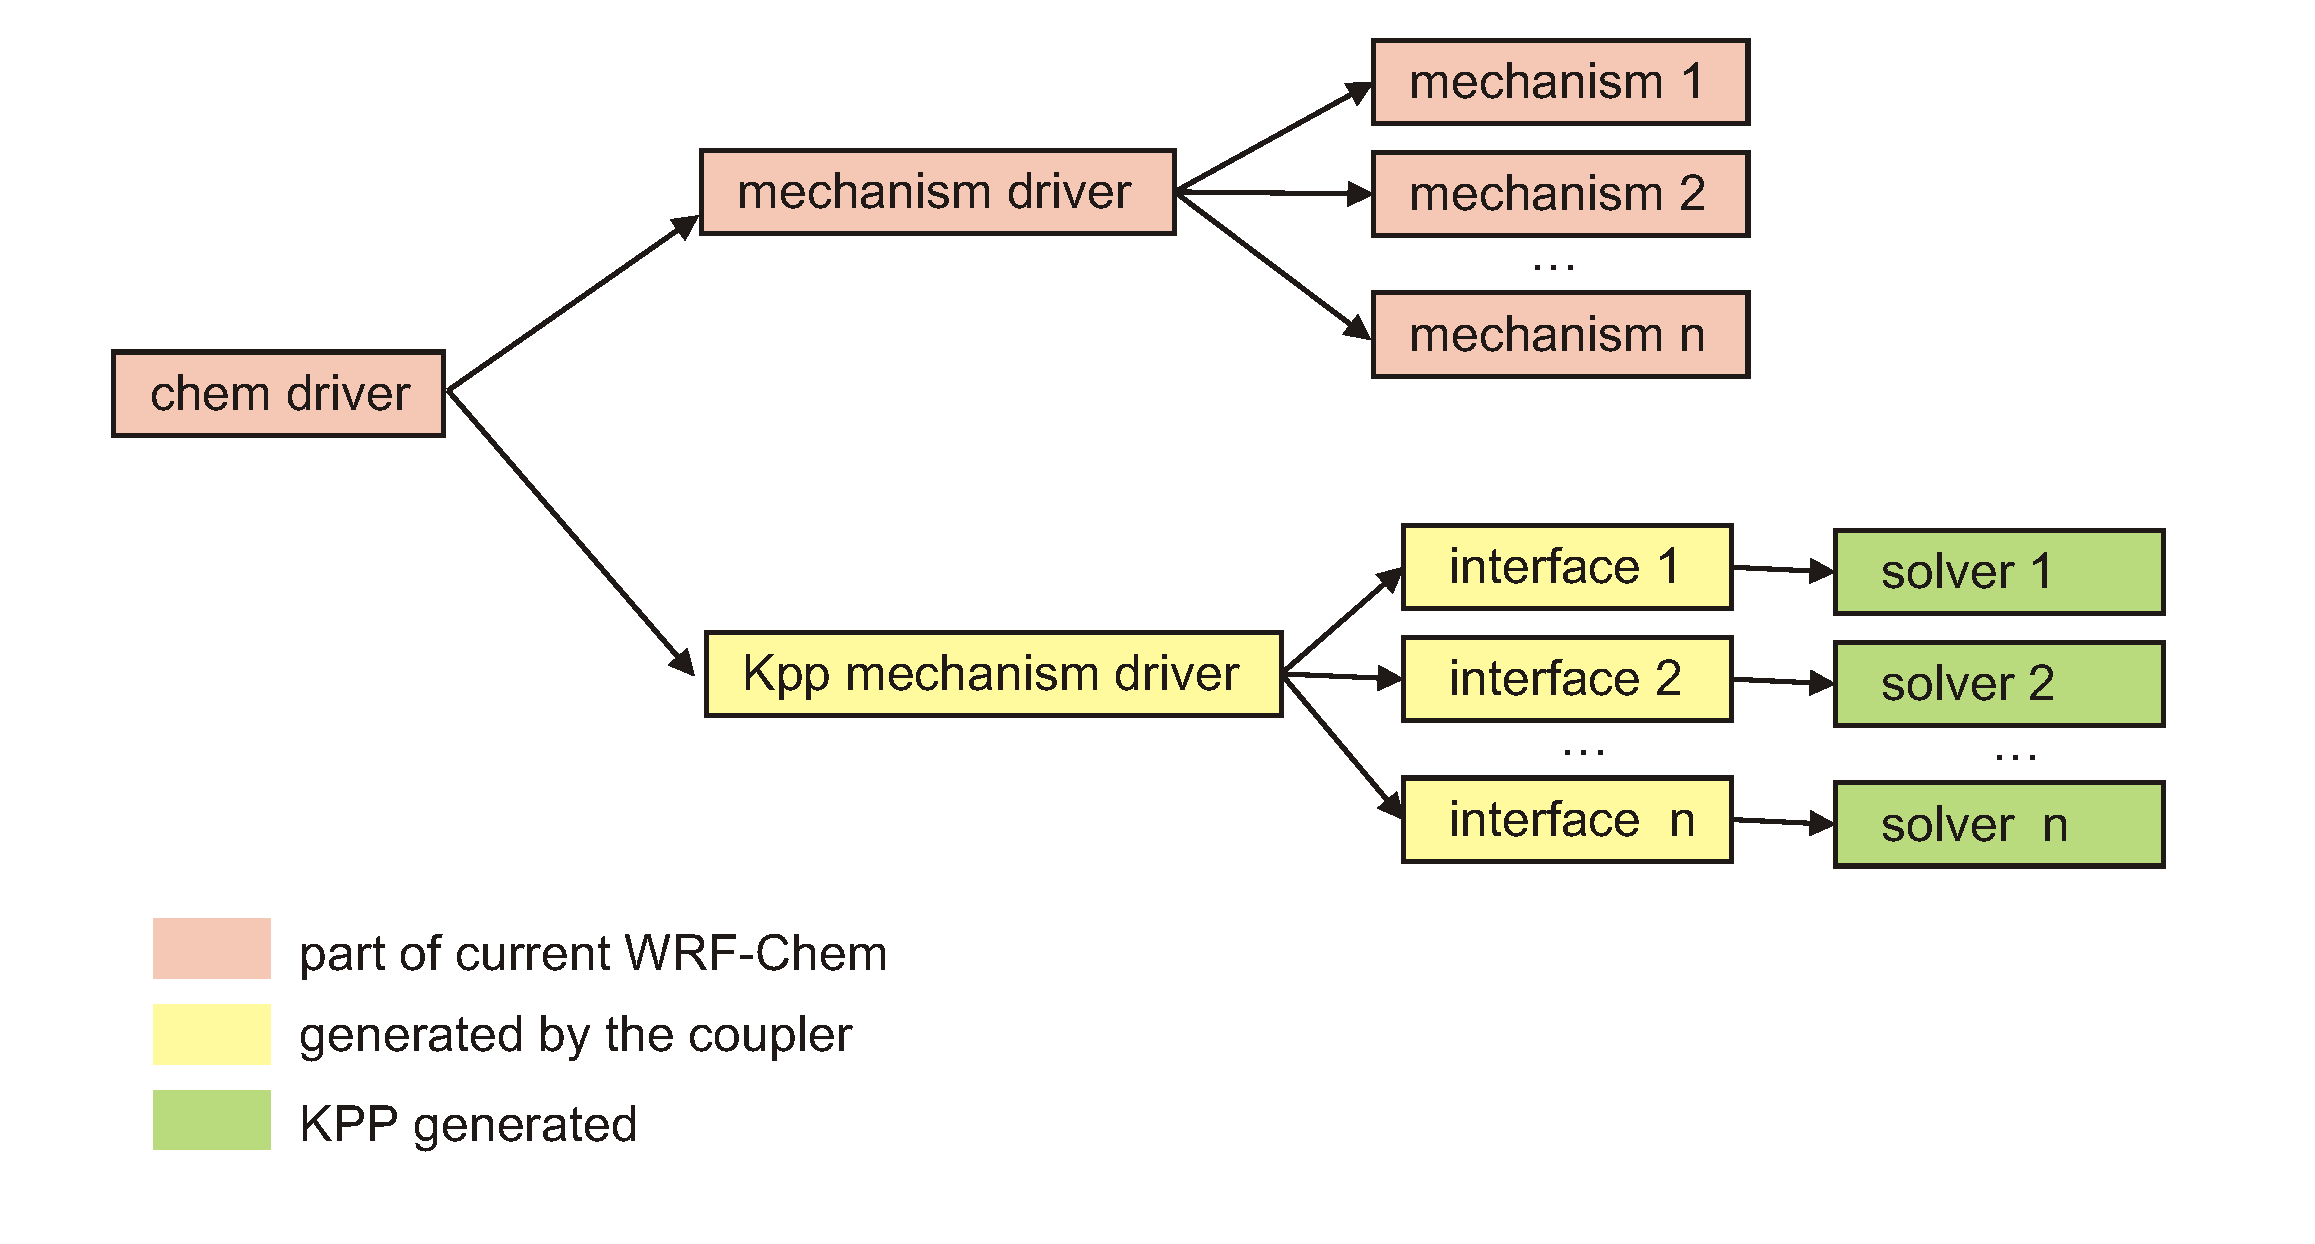
\includegraphics[width=14cm]{figs/mech_4}  
  \end{center}
  \caption{\label{fig:call} Call tree: The mechanism driver from WRF-Chem calls a separate mechanism driver for the mechanisms implemented with KPP. This setup requires only one call to be added in WRF-Chem and allows switching between mechanisms implemented with KPP and the other mechanisms in WRF-Chem.}
\end{figure} 








\section{Available integrators}

References for the chosen integrator can e.g. after compiling WRF-Chem with KPP  be found in the {\tt chem} directory in {\tt module\_kpp\_my\_mechanism\_Integrator.f90}, where {\tt ``my\_mechanism''} refers to the mechanism chosen in the WRF-Chem namelist. Currently, only Rosenbrock type integrators are available for the use with WKC. See Section \ref{sec:add_int} on how to add additional integrators.


\section{Adding additional mechanisms with WKC}\label{sec:add_mech}
The following basic steps are necessary in order to add an additional mechanism:\begin{V0}
\item edit the {\tt Registry.EM\_CHEM} to 
  \begin{V1}
  \item add additional species to the {\tt chem} array (only if necessary!). 
  \item add a package (=a mechanism) with a name ending on ``{\tt \_kpp}'', e.g. {\tt my\_mechanism\_kpp}.
  \end{V1}
\item provide input files {\tt my\_mechanism.eqn}, {\tt my\_mechanism.spc}, {\tt my\_mechanism.kpp} for KPP in a sub-directory of {\tt chem/KPP/mechanisms} named after the package (i.e. {\tt my\_mechanism}, not  {\tt my\_mechanism\_kpp}).  
\item optionally provide a file ({\tt my\_mechanism\_wrfkpp.equiv}) for mapping variable names in WRF to variable names in KPP (e.g. HO to OH).  
\end{V0}
For examples, see mechanisms which have already been implemented. When copying one of the directories in {\tt chem/KPP/mechanisms} to another directory it is necessary to change the name of {\tt \#Model} in the {\tt .kpp} file and the names of the {\tt .eqn} and the {\tt .spc} file in the {\tt .def} file. When introducing a ``new'' {\tt .kpp} file set the {\tt \#INTEGRATOR} to an integrator contained in the directory {\tt chem/KPP/kpp/kpp-2.1/int/WRF\_conform}, e.g.\smallskip \\
{\tt \#INTEGRATOR WRF\_conform/rosenbrock}\smallskip\\
and add\smallskip\\
{\tt \#WRFCONFORM}\smallskip\\
to the {\tt .kpp} file. Note, that not all KPP options are supported by WKC. Furthermore, WKC is currently not able to handle comments in the {\tt .spc} file! 

\subsection{Adding a package to the Registry}
 Is pretty straight forward.

\subsection{Adapting KPP equation files and using the wrf\_kpp\_equiv file for mapping species names}
Adapting a KPP equation file for the use with WRF involves renaming a few variables in the equation file: \\ 
\begin{tabular}{|l|c|c|c|}
\hline
                 & KPP {\tt .eqn} file & unit in { \tt .eqn} file & Registry  \\
\hline
Photolysis rate (e.g.) &j(Pj\_no2))        & s$^{-1}$  & ph\_no2    \\
temperature            & TEMP                 &  K & t\_phy \\ 
third body conc. &   C\_M         & (molec moist air)/cm$^3$ & calculated from rho\\
water vapor conc. &  C\_H2O        & molec/cm$^3$ & calc. from  QVAPOR \\  
\hline
\end{tabular}


%wrf\_kpp\_equiv

\begin{File*}[tbp]
\begin{fminipage}
\vspace{5mm}
\begin{verbatim}
   #EQUATIONS { racm-mim  }
   {001} NO2+hv=O3P+NO  : j(Pj_no2)  ;
   {002} O3+hv=O1D{+O2} : j(Pj_o31d) ;
   ...
   {242} MACP+HO2=MAHP				: ARR2( 1.82e-13 , -1300.0, TEMP ) ; 
   {243} MACP+MACP=HACE+MGLY+0.5 HCHO+0.5 CO+HO2 	: 2.00e-12 ;  
   {244} MSACP+NO2=MPAN				: TROE( 9.70e-29 , 5.6 , 9.30e-12 , 1.5 , TEMP, C_M) ;
   ...
\end{verbatim}
\vspace{1mm}
\end{fminipage}
\caption{\label{fi:eqn} Excerpt from the KPP equation ({\tt .eqn}) file for the RACM-MIM \citep{gei03} mechanism.  }
\end{File*}

\vspace{3mm}

Photolysis rates, temperatures, third body concentrations, and water vapor concentrations are passed down from the WRF-Chem/KPP interface routines. Photolysis rates are stored pointwise in a 1-D array and addressed by pointers defined in the automatically generated interface routine. For example, the NO$_2$ photolysis rate {\tt ph\_no2} in the Registry.EM\_CHEM becomes {\tt j(Pj\_no2)} in the KPP equation file (see example in Example File~\ref{fi:eqn}).
Additional variables (e.g. user calculated N$\rm_2$O$\rm_5$ hydrolysis rates) can be passed down by modifying {{\tt .inc} files in the {\tt chem/KPP/inc} directory.

%Other pre-defined variable names are





\section{Adapting additional KPP integrators for WKC}\label{sec:add_int}
Currently, only Rosenbrock type solvers have been adapted for the use 
with the WKC. Adapting additional integrators which come
with KPP is, however, rather straight forward (but can nevertheless be time consuming). The integrator files which
come with KPP are located in the directory {\tt chem/KPP/kpp/kpp2.1/int}.
Integrators which have been adapted for WRF-Chem are located in a subdirectory 
of {\tt chem/KPP/kpp/kpp2.1/int} named {\tt WRF\_Conform}. In order to adapt an additional solver for WRF-Chem:
\begin{itemize}
\item Copy the {\tt .f90} and the {\tt .def} file to the {\tt WRF\_Conform} directory. 
\item Add {\tt KPP\_ROOT} as a prefix to the names of the subroutines in all subroutine and end subroutine statements. 
\item Change the arguments in the {\tt SUBROUTINE (KPP\_ROOT\_)INTEGRATE} statements to match the calling routine (for an example, see the existing integrator routines).
\item Remove all the {\tt USE} statements in which non-constant data is used. Instead pass down the data in the subroutine statements. This can be time consuming.
\end{itemize}

Depending on the solver, additional steps may be necessary.


\section{Installing WKC into an existing WRF-Chem version}
If you received this documentation together with WRF-Chem, WKC is already
installed, and you can skip this section. Otherwise:
\begin{itemize}
\item  Untar the {\tt chem/KPP} directory into your WRF-Chem. 
\item  Update your Registry (see {\tt Registry/Registry.EM\_CHEM} for an example).
\item  Add the following lines to the beginning of the WRF compile script (after where configure.wrf is written):
\begin{verbatim}
  setenv WRF_KPP 1
  if ( ! $?WRF_KPP )   setenv WRF_KPP  0
  if ( $WRF_KPP == 1 ) then
  chem/KPP/compile_wkc
  endif
\end{verbatim}
\item Add the following lines to the end of the WRF clean script:
\begin{verbatim}
  if ( -e chem/KPP )then
    ( cd chem/KPP; clean_kpp ) 
  endif
\end{verbatim}
\item Add a call to {\tt chem\_driver.F}:
\begin{verbatim}
  CALL kpp_mechanism_driver(   chem,                        &
    grid%id,dtstepc,config_flags,                         & 
    p_phy,t_phy,rho,moist,                                &
    vdrog3, ldrog,                                        &
!                    
#include <call_to_kpp_mech_drive.inc>
!
     ids,ide, jds,jde, kds,kde,                          &
     ims,ime, jms,jme, kms,kme,                          &
     grid%i_start(ij), min(grid%i_end(ij),ide-1),      & 
     grid%j_start(ij), min(grid%j_end(ij),jde-1),      & 
     k_start    , min(k_end,kde-ksubt)                   )  
    
\end{verbatim}

\end{itemize}

\section{Final Remarks}
If you find it necessary to make changes to the coupler, or you have implemented a new mechanism, I would appreciate your feedback (salzmann@mpch-mainz.mpg.de).  


\bibliographystyle{ms}
\bibliography{wkc}

\end{document}
